\chapter{Theory}
This section explains the theory behind the effects that has been used in the implementation. 

\subsection{Sampling}

Sampling and quantizing is used as a way to convert analog signals into digital. Sampling is discretizing the time variable. Meaning splitting the continuous signal into discrete signals, by isolating values at regularly spaced time intervals. Quantizing is the same operation but done for the pressure signal, which represents the displacement of microphones diagram from its resting place, these value range from -1 to 1.

When the signals have been converted into discrete signals they can be split up into samples. Sample being a value or sometimes a set of values in time. The average amount of samples that each second is split up into depends on the goal and use of the signal. This is called the sampling rate/frequency(Hz) and generally speaking the higher the sampling rate the wider range of sounds can be heard and the signal is higher quality. However after it passes a certain threshold human ears cannot tell the difference. If a sampling rate which is high compared to the frequency of the signal is used, the outcome signal is of good quality  since there are several samples to represent each period of the signal. If an increasingly smaller sampling rate is used on the same signal then at one point there will not be enough samples representing each period to give the correct representation of the signal’s frequency. An example can be seen in Figure \ref(Sampling) showing how a smaller sampling rate than the signal’s frequency is used and creates a signal with lower frequency than the original.

\begin{minipage}{\linewidth}% to keep image and caption on one page
\makebox[\linewidth]{%        to center the image
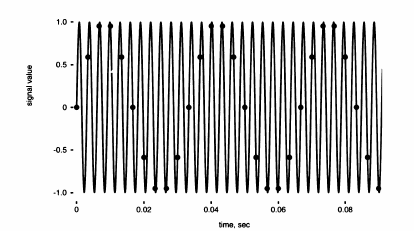
\includegraphics[keepaspectratio=true,scale=1]{Sampling}}
\captionof{figure}{Sampling a 330 Hz signal at the rate of 300 Hz\citep{Steiglitz[pp. 44]}}\label{Sampling}
\end{minipage}\\

The most common sampling rate used when it is needed to capture the entire range of human hearing(20-20000 Hz) are 44.1 kHz(same as used in compact discs), 48 kHz, 88, and 96 kHz. The reason for a sample rate to be twice as high as the signal’s frequency is due to the Nyquist theorem which claims that a double rate is enough to perfectly reconstruct the signal. While it is possible to reconstruct a signal without the double sampling rate, other constraints of the signal need to be known. For the prototype a sampling rate of 48 kHz was chosen. A higher sampling rate is not necessary as a higher sampled signal than 50 kHz does not provide any additional information to a human listener. A lower sampling frequency as 44.1 kHz could be used with the same effects, but one lower than that should not be used.

\subsection{Pitch Shift}

The first pitch shifters were built based on the principle of a rotating tape heads \citep{Katjaas_00}. They were used in the 60's to change e.g. radio interviews, so they could speed up the interview, but still maintain the same pitch. They used six tape heads to read the normal tape that you want to pitch shift at a speed independent from the tape speed. The speed of the tape head determined the duration of the sound, and the direction of tape heads controlled the pitch shift. When the head rotates in the same direction as the tape, the pitch is lowered and if it rotates in the other direction, the pitch is increased, as seen in figure \ref{TapeHead}. \\

\begin{minipage}{\linewidth}% to keep image and caption on one page
\makebox[\linewidth]{%        to center the image
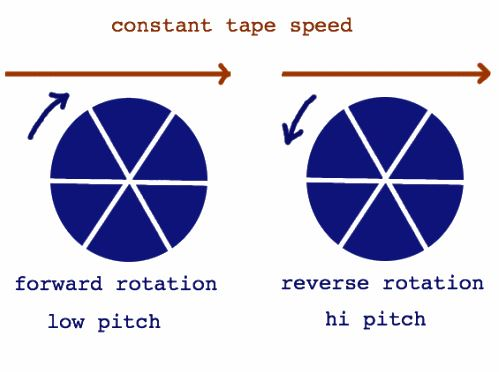
\includegraphics[keepaspectratio=true,scale=1]{TapeHead}}
\captionof{figure}{Graphical Impression of the tape head principle\citep{Katjaas_00}}\label{TapeHead}
\end{minipage}\\

The first pitch shifters used six tape heads, but digitally you only need two. If you want to raise the pitch by e.g. three semitones, how much faster must the tape reader go?
This equation converts the semitone number to a "tape reader speed" number:

\[ 2^{h/12} = e^{0.05776*h} \] where h is the halftone number. E.g. three halftones would give the "tape head reader speed" number 1.189. \\

This means that we have a tape playing at a speed of one, and a tape head reader reading at a speed of 1.189. \\

In a digital setting the tape heads are replaced with two read pointers that change their delay depending on the required pitch shift. Increasing the delay when lowered pitch is needed and decreasing it if a raised pitch is needed. 
The read pointer will at some point pass the write pointer, because of the delay. When this happens a click can be heard if audio from only one read point is played. To combat this the cos~ object is used which creates a smooth crossfade to the second read pointer.

\subsection{Harmonise}

A harmony is a sound created by playing or singing different notes at the same time\citep{Harmonise02}.
Singing harmony means that a backup vocalist or someone else is singing the needed notes in conjunction with the lead singer singing the main melody notes. In a digital setting this effect can be achieved with a single voice. This is done by pitch-shifting the voice multiple times, each time with a different shift in semitones and stacking them together creating the effect of singing in harmony. 
A chord or a harmony is multiple notes, usually three or more, played at the same time. A chord in which three notes are played is called a "triad"\citep{Harmonise01}. A triad is build on thirds, a root, a third, and a fifth note, see figure \ref{triadPic}. The third being a third above the root and fifth being a third above third, or a fifth above the root. Depending on the quality of the two third intervals the quality of the triad changes. \\

\begin{minipage}{\linewidth}% to keep image and caption on one page
\makebox[\linewidth]{%        to center the image
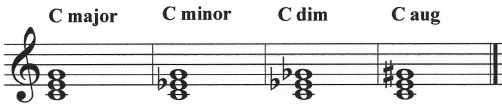
\includegraphics[keepaspectratio=true,scale=1]{triad}}
\captionof{figure}{A major, minor, diminished, and a augmented triad \citep{triad}}\label{triadPic}
\end{minipage}\\

In western music there are seven kinds of harmonies, three major, three minor and one diminished. The major triad and the minor triad will be implemented in the program of this project.